\documentclass[a4paper,12pt]{report}
\usepackage[utf8]{vietnam}
\usepackage{graphicx}
\usepackage{fancybox}
\usepackage{longtable}
\usepackage{listings}
\usepackage{xcolor}
\usepackage{hyperref}
\usepackage{titlesec}
\usepackage{mdframed}
\usepackage{amsmath}
\usepackage{array}
\newmdenv[linecolor=black,skipabove=\topsep,skipbelow=\topsep,
leftmargin=-5pt,rightmargin=-5pt,
innerleftmargin=5pt,innerrightmargin=5pt]{mybox}
\usepackage[left=3cm, right=2.00cm, top=2.00cm, bottom=2.00cm]{geometry}
\lstset{language=java,
   %keywords={break,case,catch,continue,else,elseif,end,for,function,
   %   global,if,otherwise,persistent,return,switch,try,while},
   basicstyle=\ttfamily \fontsize{8}{10}\selectfont,   
	% numbers=left,
   frame=lrtb,
tabsize=3
}
\usepackage{hyperref}  
\hypersetup{
    colorlinks,
    citecolor=black,
    filecolor=black,
    linkcolor=black,
    urlcolor=black
}


\newcommand{\ig}{\includegraphics}
\usepackage{tabularx}
\newcolumntype{L}[1]{>{\raggedright\arraybackslash}p{#1}}
\newcolumntype{C}[1]{>{\centering\arraybackslash}p{#1}}
\newcolumntype{R}[1]{>{\raggedleft\arraybackslash}p{#1}}
\begin{document}
\thispagestyle{empty}
\thisfancypage{
\setlength{\fboxrule}{1pt}
\doublebox}{}
\begin{center}
{\fontsize{16}{19}\fontfamily{cmr}\selectfont TRƯỜNG ĐẠI HỌC BÁCH KHOA HÀ NỘI\\
VIỆN CÔNG NGHỆ THÔNG TIN VÀ TRUYỀN THÔNG}\\
\textbf{------------*******---------------}\\[1cm]

\includegraphics[scale=0.13]{hust.jpg}\\[1.3cm]

{\fontsize{32}{43}\fontfamily{cmr}\selectfont BÁO CÁO}\\[0.1cm]
{\fontsize{38}{45}\fontfamily{cmr}\fontseries{b}\selectfont MÔN HỌC}\\[0.2cm]
{\fontsize{19}{20}\fontfamily{phv}\selectfont NHẬP MÔN CÔNG NGHỆ PHẦN MỀM}\\[0.2cm]
{\fontsize{19}{20}\fontfamily{cmr}\selectfont \emph{Đề tài: Xây dựng menu điện tử phục vụ nhà hàng}}\\[2.0cm]
\end{center}
\hspace{1cm}\fontsize{14}{16}\fontfamily{cmr}\selectfont \textbf{Nhóm sinh viên thực hiện:}

\begin{longtable}{l c c}

Họ và tên & MSSV  & Lớp\\
Đỗ Thanh Bình & 20130325 & 84307 \\
Nguyễn Tuấn Đạt &  20130856 & 84307 \\
Trần Văn  Đức & 20131070 & 83444 \\
Đặng Quang Trung & 20134145  & 84307 \\
Phan Anh Tú & 20134501  & 84307 \\

\end{longtable}

\hspace{1cm}\fontsize{14}{16}\fontfamily{cmr}\selectfont \textbf{Giáo viên hướng dẫn: }TS. Nguyễn Thanh Hùng\\[2cm]
\begin{center}
\fontsize{16}{19}\fontfamily{cmr}\selectfont Hà Nội 01--2016

\end{center}
\newpage
\tableofcontents
\chapter*{Mở đầu}
\addcontentsline{toc}{chapter}{Mở đầu}
%to do
Công nghệ phần mềm là lĩnh vực được chú trọng, thu hút đông đảo kĩ sư nhất trong ngành công nghệ thông tin hiện nay. Nó đòi hỏi sự sáng tạo trong ý tưởng, nghiêm khắc trong các quy trình, chăm chỉ, bền bỉ trong công việc, và rất nhiều yếu tố khác nữa. Học phần "Nhập môn công nghệ phần mềm" là học phần tất yêu đối với sinh viên, kĩ sư công nghệ phần mềm. Được học học phần này là niềm thú vị đối với chúng em.\\

Trong quá trình học tập, chúng em đã chọn đề tài bài tập lớn "Tìm	hiểu đặc	tả yêu	cầu,	phân	tích	thiết	kế hệ thống	và	thiết	kế một	số
trường	hợp	kiểm	thử cho menu	điện	tử phục	vụ nhà	hàng (đặt	món	ăn,	huỷ món	
ăn,	báo	nhà	bếp,	thống	kê	theo	ngày)." Nhóm chúng em bao gồm:\\
\begin{longtable}{l c c}

Họ và tên & email  & Di động\\
Đỗ Thanh Bình & magic10995@gmail.com & 0167 461 1215 \\
Nguyễn Tuấn Đạt &  20130856 & 84307 \\
Trần Văn  Đức & tv.duc95@gmail.com & 0169 314 0664 \\
Đặng Quang Trung & 20134145  & 84307 \\
Phan Anh Tú & 20134501  & 84307 \\
\end{longtable}

Chúng em cảm ơn thầy đã giảng dạy học phần và hướng dẫn chúng em làm bài tập lớn.

\chapter{Giới thiệu Project}
\begin{itemize}
\item Đề tài: Xây dựng menu điện tử phục vụ nhà hàng. 
\item Mục đích: Xây dựng phần mềm cho nhân viên phục vụ, nhà bếp và thu ngân, ứng dụng công nghệ thông tin vào đời sống hàng ngày.
\item Mô tả: Tìm	hiểu đặc	tả yêu	cầu,	phân	tích	thiết kế hệ thống	và	thiết	kế một	số
trường	hợp	kiểm	thử cho menu	điện	tử phục	vụ nhà	hàng (đặt	món	ăn,	huỷ món	
ăn,	báo	nhà	bếp,	thống	kê	theo	ngày). Mô hình chi tiết sẽ trong phần đặc tả hệ thống.
\item Chi tiết:
\begin{itemize}
       \item Nhân sự: đội ngũ kỹ sư, lập trình phần mềm (4 người) và một designer.
       \item Thời gian bàn giao sản phẩm dự kiến 3 tháng.
       \item Giá thành phần mềm: 50 triệu đồng. Mỗi thiết bị andoird cho nhân viên: 4 triệu. Server: 10 triệu. PC cho thu ngân: 5 triệu. (Coi như các thiết bị cơ bản wifi, router nhà hàng đã có sẵn).
      \end{itemize}
\item Rủi ro và cách giải quyết:
\begin{itemize}
        \item{Giữ nguồn điện ổn định cho nhà hàng, có giải pháp thay thế khi mất điện.}
        \item{Sẵn sàng cập nhập server khi cơ sở dữ liệu ngày càng lớn dần.}
        \item{Thường xuyên bảo trì hệ thống, sửa lỗi phần mềm.}
      \end{itemize}
\end{itemize}


\chapter{Đặc tả}
\section{Đặc tả chức năng}
Biểu đồ luồng dữ liệu:\\
\begin{figure}[h]
\centering
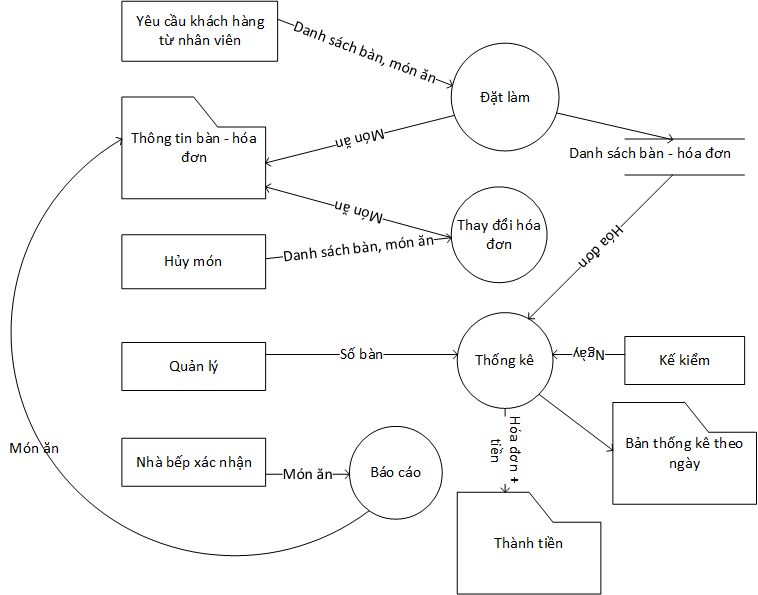
\includegraphics[scale=0.7]{DFD.png}
\caption{Biểu đồ luồng dữ liệu}
\end{figure}

\section{Đặc tả dữ liệu}
\subsection{Mô hình thực thể liên kết}
\begin{figure}
\centering
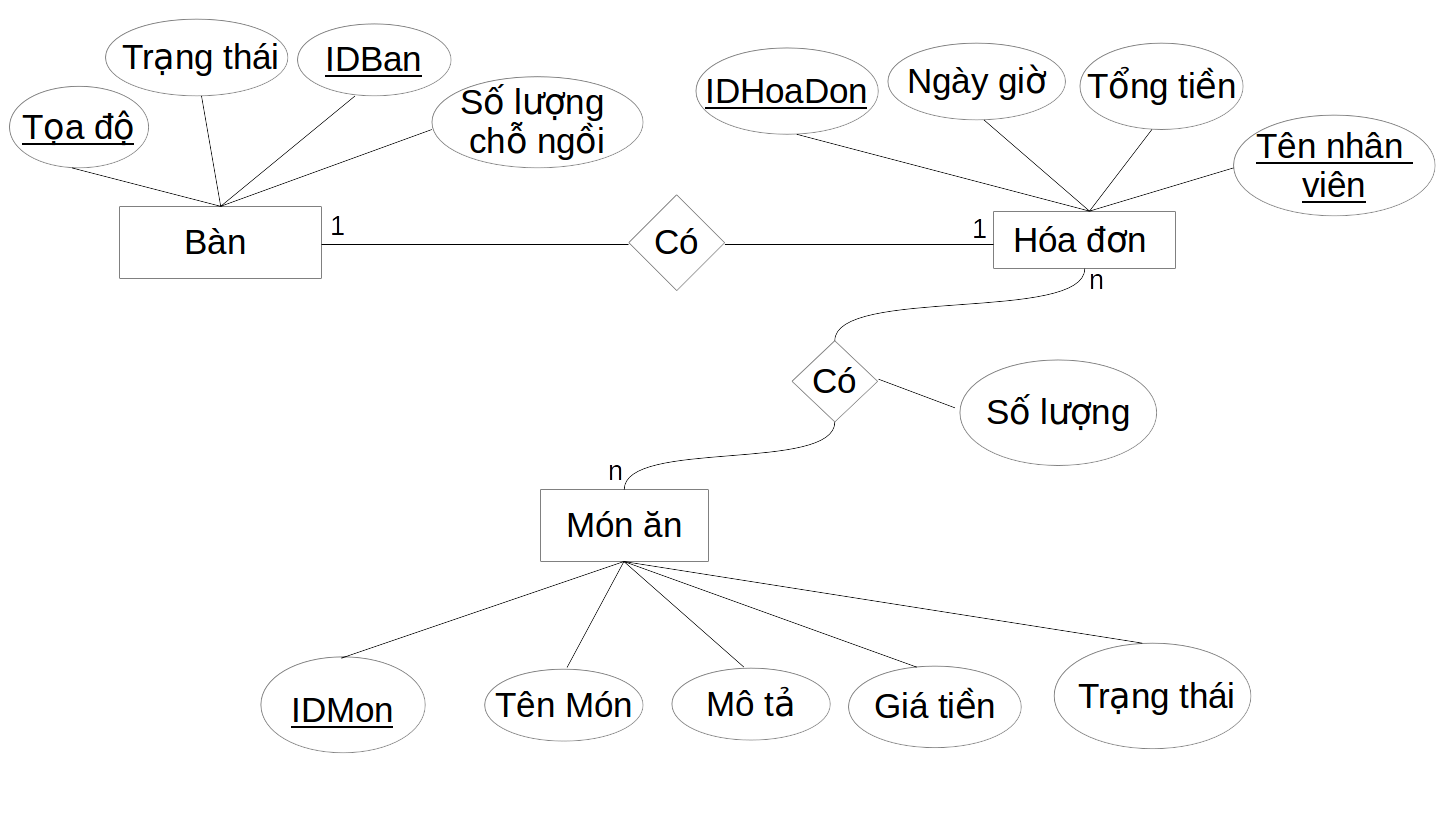
\includegraphics[scale=0.4]{DuLieu.png}
\caption{Sơ đồ thực thể liên kết}
\end{figure}
\subsection{Mô hình quan hệ (Bảng lưu trong CSDL)}
\textbf{Ban}(\underline{IDBan}, ToaDo, SoLuongChoNgoi, TrangThai, IDHoaDon)\\
\textbf{HoaDon}(\underline{IDHoaDon}, NgayGio, TongTien, TenNhanVien)\\
\textbf{MonAn}(\underline{IDMon}, TenMon, MoTa, GiaTien, TrangThai)\\  
\textbf{MonAnTheoBan}(\underline{IDHoaDon, IDMon}, SoLuong) 

\begin{itemize}
\item Bảng \textbf{Ban} bao gồm các thuộc tính \textbf{IDBan}, \textbf{ToaDo} để xác định vị trí của bàn trong nhà hàng; thuộc tính \textbf{SoLuongChoNgoi} cho biết bàn có bao nhiêu chỗ để sắp xếp khách cho phù hợp; thuộc tính \textbf{TrangThai} cho biết bàn còn trống hay đã có khách (chỉ nhận giá trị 0 hoặc 1 tương ứng với bàn còn trống và đã có khách); thuộc tính \textbf{IDHoaDon} là khóa ngoài tham chiếu đến thuộc tính \textbf{IDHoaDon} của bảng \textbf{HoaDon} để xác định hóa đơn tương ứng với từng bàn.
\item Bảng \textbf{HoaDon} bao gồm các thuộc tính \textbf{IDHoaDon} phân biệt các hóa đơn của các khách khác nhau; thuộc tính \textbf{NgayGio} cho biết hóa đơn đó được lập vào ngày nào; thuộc tính \textbf{TongTien} cho biết giá trị của hóa đơn (tổng số tiền mà khách hàng phải thanh toán), thuộc tính này có thể tính từ thuộc tính \item{GiaTien} của bảng \textbf{MonAn} nhưng để thuận tiện cho việc thống kê (tránh phải truy xuất CSDL nhiều lần) ta tách riêng thành một thuộc tính; thuộc tính \textbf{TenNhanVien} cho biết tên nhân viên lập hóa đơn.
\item Bảng \textbf{MonAn} bao gồm các thuộc tính \textbf{IDMonAn}, \textbf{TenMon} để xác định tên món ăn, thuộc tính \textbf{MoTa} để mô tả chi tiết về món ăn, thuộc tính \textbf{GiaTien} cho biết giá của món ăn đó; thuộc tính \textbf{TrangThai} cho biết nhà hàng hôm nay có món đó không (chỉ nhận giá trị 0 (tương ứng với không) hoặc 1 (tương ứng với có)).
\item Bảng \textbf{MonAnTheoBan} liệt kê danh sách các món ăn và số lượng của từng món của 1 bàn   
\end{itemize}

\chapter{Phân tích thiết kế}
\section{Phân tích yêu cầu phần mềm menu diện tử}
\begin{itemize}
	\item \textbf{Chức năng:} Đặt món ăn, hủy món ăn, báo nhà bếp, thống kê theo ngày.
	\item \textbf{Phạm vi:} nhà hàng bao gồm các bộ phận: bếp, nhà ăn, quản lý.
	\item \textbf{Kỹ thuật:} Sử dụng mạng lan wifi kết nối giữa các thiết bị, quản lý theo Id.
	\item \textbf{Đối tượng tham gia sử dụng:} Khách hàng, nhân viên phục vụ, nhà bếp và quầy quản lý.
	\item \textbf{Kịch bản:} Khách hàng ngồi tại bàn x đặt món, hủy món qua thiết bị điện tử của nhân viên,  nhân viên gửi danh sách đến nhà bếp, nhà bếp bắt đầu làm và check các món đã làm, khách hàng có thể hủy bỏ món, sau khi ăn xong, khách hàng ra quầy quản lý thanh toán. Quầy quản lý có dữ liệu tại bàn x và tính toán, thu tiền của khách.
	\item \textbf{Quy mô:} Nhiều nhân viên, nhiều bếp, nhiều bàn và nhiều quầy quản lý.
\end{itemize}
\pagebreak
\section{Thiết kế}
Mô hình hóa phần mềm với UML:
\begin{itemize}
	\item Biểu đồ Class\\
	\begin{figure}[h]
		\centering
		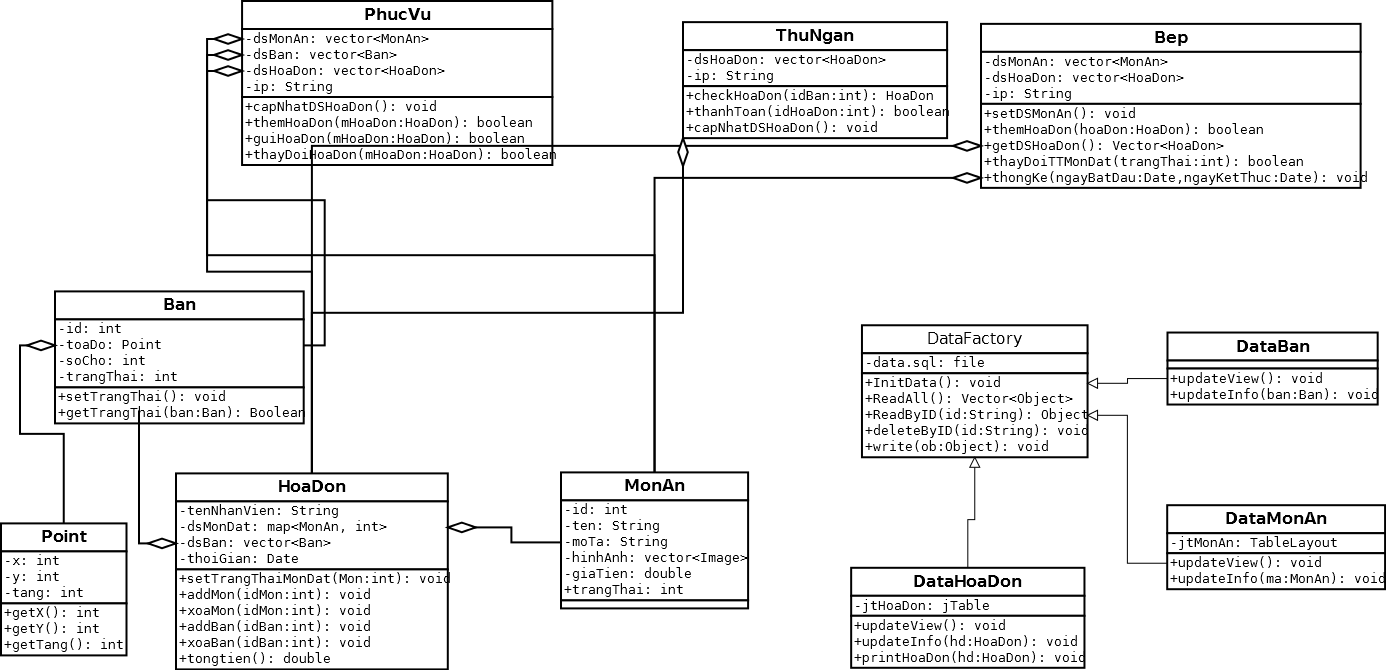
\includegraphics[scale=0.3]{UML-Final.png}
		\caption{Class - Diagram}
	\end{figure}
	\item Biểu đồ UseCase\\
	\begin{figure}[h]
		\centering
		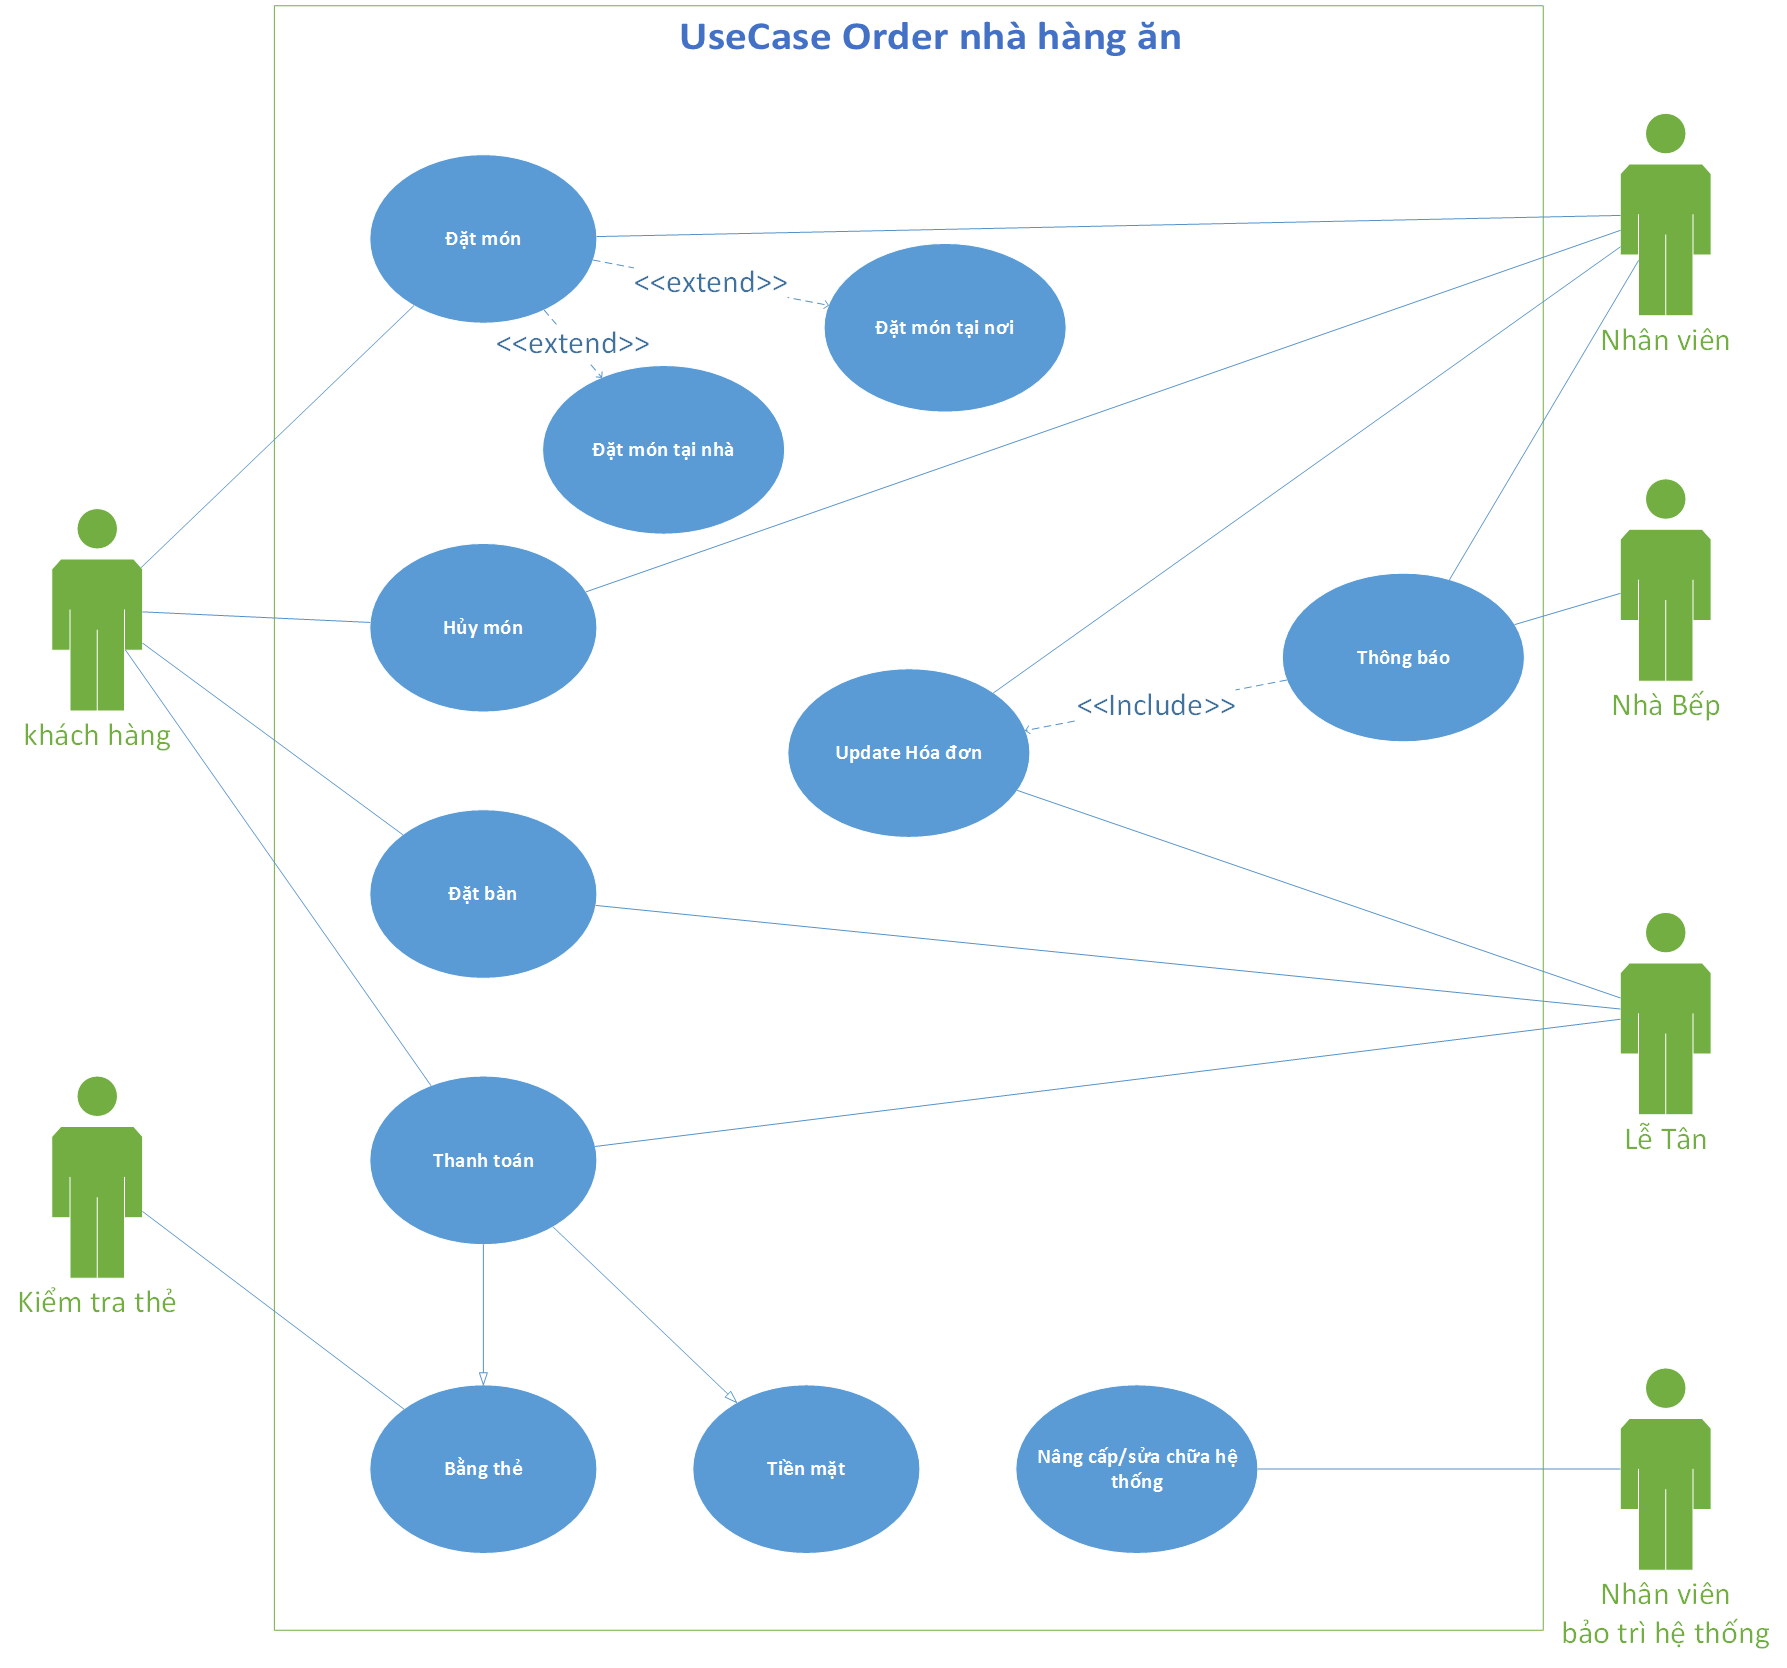
\includegraphics[scale=0.2]{UseCase.png}
		\caption{UseCase - Diagram}
	\end{figure}
\end{itemize}
\chapter{Code}
\section{Công nghệ sử dụng}
\begin{itemize}
	\item Sử dụng biểu đồ DFD, FSO và thực thể liên kết để phân tích yêu cầu.
	\\$\Rightarrow$ Dễ hiểu, trực quan cho cả khách hàng lẫn đội ngũ kĩ sư.
	\item Sử dụng biểu đồ Use-case, UML classes để thiết kế hệ thống.
	\\$\Rightarrow$ Đơn giản, quen thuộc và đầy đủ.
	\item Lập trình bằng ngôn ngữ Java, sử dụng gói Java Swing để thiết kế giao diện cho thu ngân.
	\\$\Rightarrow$ Java là ngôn ngữ hỗ trợ công nghệ hướng đối tượng mạnh, chạy đa nền tảng, phổ biến nhất hiện nay trong việc xây dựng các phần mềm.
	\\$\Rightarrow$ Java Swing hỗ trợ xây dựng giao diện nhanh, hiệu quả, hỗ trợ kéo thả.
	\item Cơ sở dữ liệu dùng hệ quản trị cơ sở dữ liệu MySQL.
	\\$\Rightarrow$ Đơn giản, chi phí thấp.
	\item Xây dựng trên nền tảng Android (mỗi nhân viên trạng bị máy tính bẳng android để giao tiếp với hệ thống), ngôn ngữ Java trên Android platform.
	\item Kết nối giữa client và server dựa vào mạng wifi, đặt ip tĩnh cho các thiết bị.
	\\$\Rightarrow$ Nhẹ nhàng, linh động.
	\\ Trao đổi thông tin giữa client và server thông qua socket, giao thức TCP.
	\\ Socket là một cổng logic nằm giữa process ứng dụng và end-transport protocol. Có hai loại socket thường dùng là Stream Socket (dựa trên giao thức TCP) và Datagram Socket (dựa trên giao thức UDP). Một TCP/IP socket bao gồm một địa chỉ IP và một cổng. Địa chỉ IP dùng để xác định máy tính trên mạng còn cổng được sử dụng để xác định tiến trình.
	\\ Ở đây ta sử dụng giao thức TCP để đảm bảo dữ liệu truyền đến nơi nhận một cách đáng tin cậy và đúng thứ tự.
	\\ Giải thuật cho client:
	\\ \hspace*{3mm} - Xác định địa chỉ server
	\\ \hspace*{3mm} - Tạo socket
	\\ \hspace*{3mm} - Kết nối đến server
	\\ \hspace*{3mm} - Gửi nhận dữ liệu
	\\ \hspace*{3mm} - Đóng kết nối
	\\ Giải thuật cho server
	\\ \hspace*{3mm} - Tạo socket, đăng ký với hệ thống
	\\ \hspace*{3mm} - Đặt socket ở chế đọ chờ, lắng nghe kết nối
	\\ \hspace*{3mm} - Khi có request từ client, chấp nhận kết nối, tạo một process con để xử lí. Quay lại trạng thái chờ, lắng nghe kết nối mới.
	\\ Công việc của process con
	\\ \hspace*{3mm} - Nhận thông tin kết nối từ client
	\\ \hspace*{3mm} - Giao tiếp với client
	\\ \hspace*{3mm} - Đóng kết nối và kết thúc process con
	\\
	\\ $\Rightarrow$ An toàn, bảo mật, tiện dụng.
	
\end{itemize}
\chapter{Kiểm thử}
\section{Kiểm thử hộp đen}
Đối tương kiểm thử là một modular thu ngân trong hệ thống order phục vụ nhà hàng ăn.
\subsection{Phân tích đặc tả về các yêu cầu chức năng của modular thu ngân cần thực hiện.}
Modular thu ngân là một modular thanh toán tiền cho khách hàng gồm có chức năng chính:
\begin{itemize}
\item Kiểm tra hóa đơn của khách hàng thông qua dữ liệu vào là \textbf{idban} và trả về hóa đơn tương ứng với bàn đó.
\item Thanh toán hóa đơn đầu vào là \textbf{idhoadon} và trả về kết quả đã thanh toán hay chưa.
\end{itemize}
\subsection{Sử dụng kĩ thuật kiểm thử phân lớp tương đương để định nghĩa các testcase của các chức năng trên}
Mỗi lần có khách thanh toán, modular thu ngân sẽ thực hiện các chức năng trên và đưa ra kết quả theo bảng sau:\\
\textbf{•} Chức năng kiểm tra hóa đơn:
\begin{itemize}
\item[-] Dữ liệu vào là idban.
\item[-] Kết quả mong muốn là hóa đơn tương ứng với bàn đó.
\end{itemize}
\begin{longtable}{|c|c|}
\hline
\textbf{ID Bàn}   			& \textbf{Kết quả mong đợi} \\
\hline
\textbf{<1} &\textbf{ Lỗi} \\
\hline
\textbf{1 - 100} & \textbf{Hóa đơn tương ứng với ID bàn.} \\
\hline
\textbf{>100} & \textbf{Lỗi}\\
\hline
\textbf{String} & \textbf{Lỗi}\\
\hline
\end{longtable}
\textbf{•} Chức năng thanh toán:
\begin{itemize}
\item Dữ liệu vào là ID hóa đơn.
\item Dữ liệu đầu ra thanh toán thành công hay chưa(true/false)
\end{itemize}
\begin{longtable}{|c|c|}
\hline
\textbf{ID hóa đơn}   			& \textbf{Kết quả mong đợi} \\
\hline
\textbf{< 1} &\textbf{ Chưa thanh toán thành công} \\
\hline
\textbf{$\geq$ 1} & \textbf{Hóa đơn tương ứng với ID bàn.} \\
\hline
\textbf{String} & \textbf{ Chưa thanh toán thành công}\\
\hline
\end{longtable}
\subsection{Kiểm thử các testcase đã định nghĩa}
Với mỗi trường hợp ta lấy đại diện thay vì kiểm tra hết các trường hợp.\\
\\
\textbf{•} Chức năng kiểm tra hóa đơn: lấy các testcase đại diện sau
\begin{itemize}
\item[1.] test1 \{ input = 0,output = lỗi \}
\item[2.] test2 \{ input = 1,output = Hóa đơn \}
\item[3.] test3 \{ input = 101,output = lỗi \}
\item[4.] test4 \{ input = String,output = lỗi \}
\end{itemize}
\textbf{•} Chức năng thanh toán: lấy các testcase đại diên sau
\begin{itemize}
\item[1.] test1 \{ input = 0,output = chưa thanh toán thành công \}
\item[2.] test2 \{ input = 1,output = thanh toán thành công \}
\item[3.] test3 \{ input = String,output = thanh toán chưa thành công \}
\end{itemize}
\subsection{So sánh kết quả thu được với kì vọng(lập bảng)}
\begin{itemize}
\item chức năng kiểm tra hóa đơn (KTHD)
\item chức năng thanh toán(TT)
\end{itemize}
\newpage
\begin{longtable}{|L{2cm}|L{2.5cm}|L{3.1cm}|L{3.1cm}|L{2.5cm}|L{1.5cm}|}
\hline
\textbf{Testcase ID}   & \textbf{Testcase description} & \multicolumn{2}{c|}{ \textbf{Testcase procedures}               } & \textbf{Testcase} & \textbf{Status}      \\ 
\cline{3-4}
 &  &\textbf{ Step to} & \textbf{Step} & \textbf{Expected} &  \\ 
 &  &\textbf{perform} & \textbf{Expected} & \textbf{Result} &  \\ 
 &  &  & \textbf{Result} &  &  \\ 
 &  &  &  &  &  \\ 
 &  &  &  &  &  \\ 
\hline
KTHD1 &  Kiểm tra lỗi hóa đơn khi idban là số nguyên < 0& Điên giá trị idban $\leq$ 0(-1) vào filed có nhã idban rồi click vào nút kiểm tra & Kết quả thu được màn hình báo lỗi(Không có bàn đó)&  &  \\ 
\hline
KTHD2 &  Kiểm tra đưa ra hóa đơn khi idban 1-100 & Điên giá trị 0 $\leq$ idban $\leq$ 100(10) vào filed có nhã idban rồi click vào nút kiểm tra & Kết quả thu được màn hình đưa ra 1 hóa đơn tương ứng với bàn đó&  &  \\ 
\hline
KTHD3 &  Kiểm tra lỗi hóa đơn khi idban là số nguyên > 100& Điên giá trị idban > 100(102) vào filed có nhã idban rồi click vào nút kiểm tra & Kết quả thu được màn hình báo lỗi(Không có bàn đó)&  &  \\ 
\hline
KTHD4 &  Kiểm tra lỗi hóa đơn khi idban là một kí tự hoặc xâu kí tư khác số nguyên & Điên giá trị idban là xâu kí tự hoặc kí tự khác sô nguyên(abc)vào filed có nhã idban rồi click vào nút kiểm tra & Kết quả thu được màn hình báo lỗi(Không có bàn đó)&  &  \\ 
\hline
TT1 &  Kiểm tra lỗi thanh toán hóa đơn không thành công đầu vào là số nguyên < 1 &Ấn nút thanh toán điền vào trường field có nhãn idhoadon < 1(0) vào rồi click 'Ok'& Kết quả thu được màn hình báo chưa thanh toán thanh công &  &  \\ 
\hline
TT2 &  Kiểm tra lỗi thanh toán hóa đơn  thành công đầu vào là số nguyên $\geq$ 1 &Ấn nút thanh toán điền vào trường field có nhãn idhoadon $\geq$ 1(10) vào rồi click 'Ok'& Kết quả thu được màn hình báo chưa thanh toán thanh công &  &  \\ 
\hline
TT3 &  Kiểm tra lỗi thanh toán hóa đơn không thành công đầu vào là xâu hoặc chuỗi kí tự khác số nguyên &Ấn nút thanh toán điền vào trường field có nhãn idhoadon một xâu hoặc kí tự khác số nguyên(abc) vào rồi click 'Ok'& Kết quả thu được màn hình báo chưa thanh toán thanh công &  &  \\ 
\hline
\end{longtable}
\chapter{Kết luận}
Hệ thống menu điện tử xây dựng còn khá hạn chế, đối với từng mô hình nhà hàng khác nhau cần sửa đổi nhiều về nhân sự, kích thước bàn,...Ngoài ra, trong quá trình code sẽ phát sinh ra rất nhiều trường hợp, tiểu tiết mà chúng em chưa xét đến được.\\

Qua bài tập lớp này, chúng em đã rèn luyện được kiến thức:
\begin{itemize}
	\item Làm việc nhóm, kỹ năng quản lý dự án thông qua github.com.
	\item Bổ trợ kỹ năng phân tích, thiết kế hướng đối tượng.
	\item Phát triển dự án theo hệ thống, từng bước một: phân tích, đặc tả, thiết kế, lập trình, kiểm thử. 
	\item Sử dụng các công cụ, biểu đồ trong từng khâu thiết kế như DFD, FSO, Use-case, UML classes.
\end{itemize}


\chapter{Version Control}
\begin{center}
\hyperref[label_name]{https://github.com/peace195/NMCNPM}\\
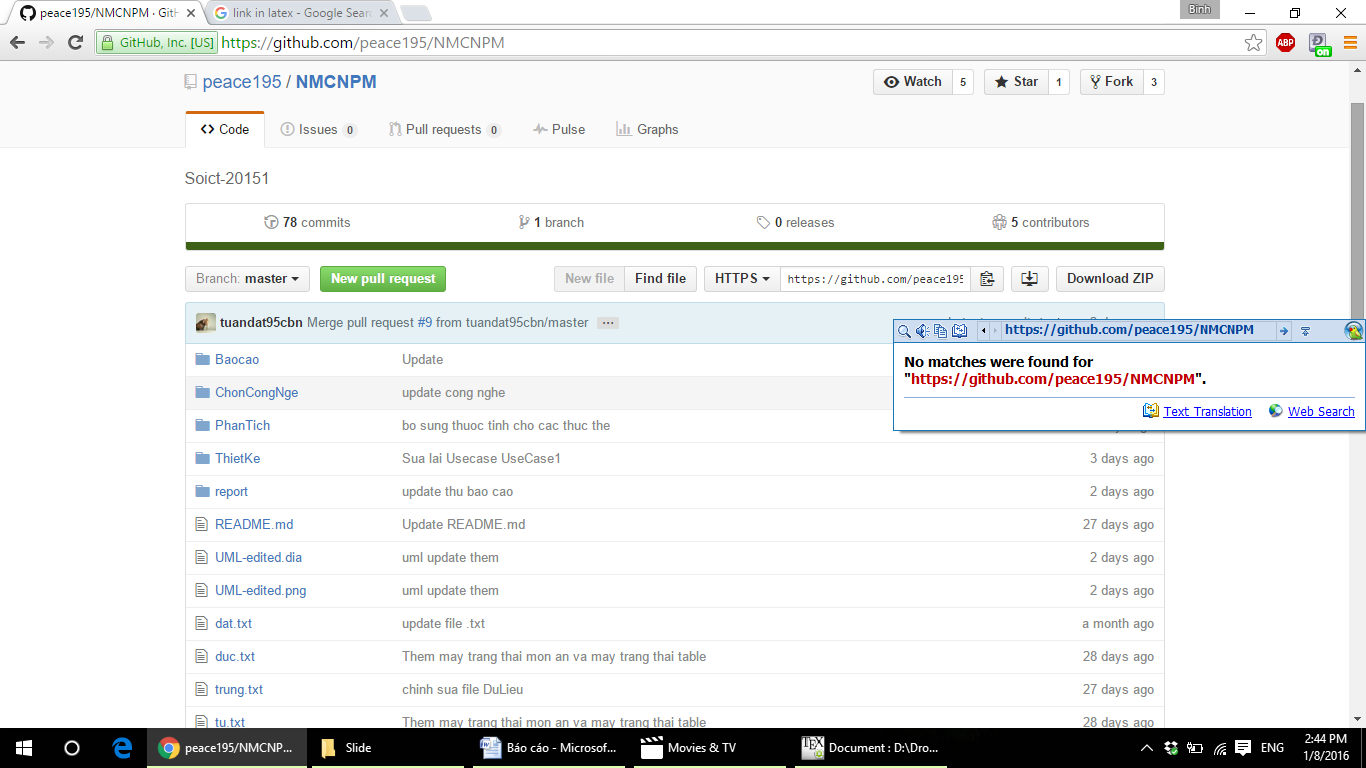
\includegraphics[scale=0.4]{vc1.png}\\
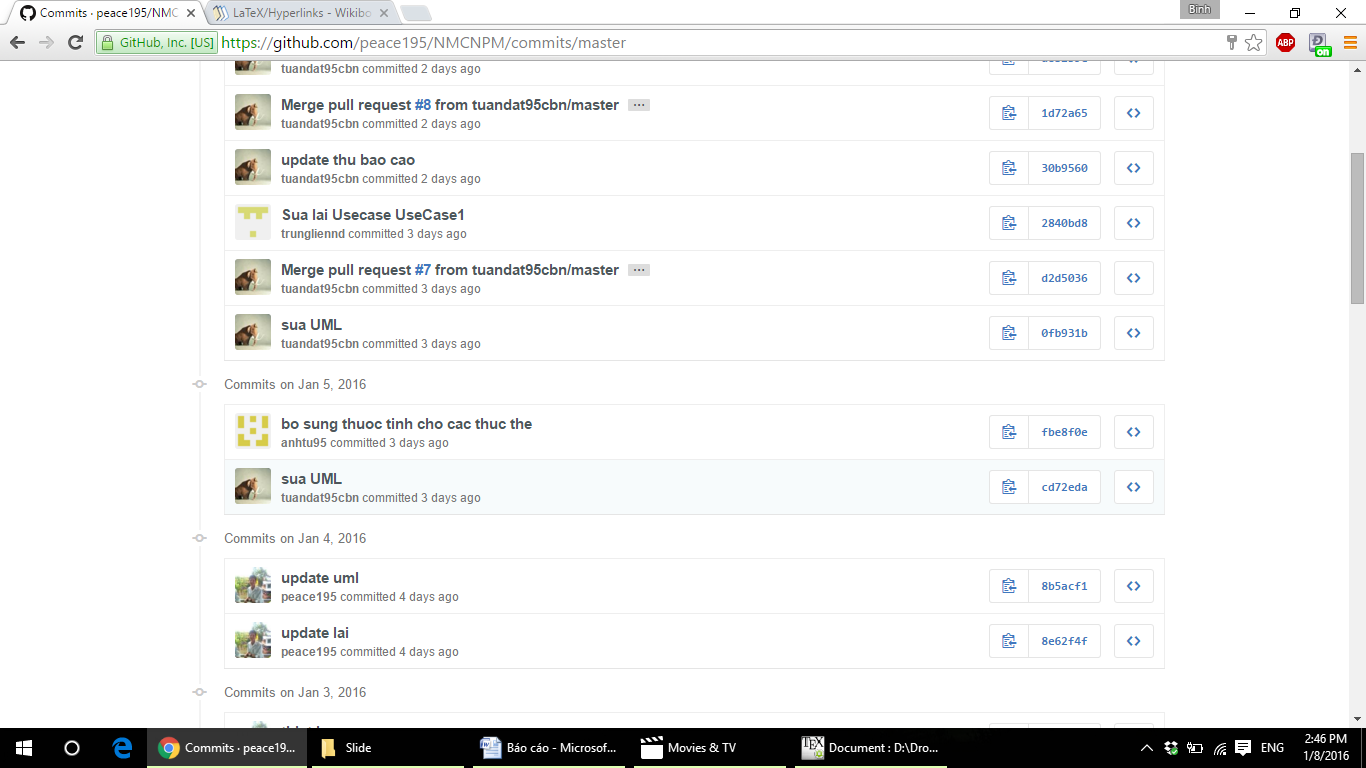
\includegraphics[scale=0.4]{vc2.png}
\end{center}
\chapter*{Tài liệu tham khảo}
\phantomsection
\addcontentsline{toc}{chapter}{Tài liệu tham khảo}
[1] Slide "Nhập môn công nghệ phần mềm", TS.Nguyễn Thanh Hùng
\end{document}
